
%(BEGIN_QUESTION)
% Copyright 2012, Tony R. Kuphaldt, released under the Creative Commons Attribution License (v 1.0)
% This means you may do almost anything with this work of mine, so long as you give me proper credit

In the act of turning a wind turbine's rotor, wind also exerts a horizontal force on the supporting tower.  To stabilize the wind turbine tower, ``guy'' wires are attached near the top of the tower to anchor points on the ground:

$$\includegraphics[width=15.5cm]{i02585x01.eps}$$

Suppose that a wind is exerting 800 Newtons of horizontal force on the tower, measured at the point of connection between the guy wire and the tower.  This connection point is 30 meters from ground level, and the angle of the guy wire to the ground is 40$^{o}$.  Assuming that the single guy wire is bearing the full load of this wind force, how many Newtons of tension will this guy wire experience?

\vskip 10pt

$F_{tension}$ = \underbar{\hskip 50pt} lbs

\vskip 10pt

Supposing we are interested in minimizing the amount of tension the guy wire must bear, should we re-locate the concrete anchor closer to the base of the wind turbine tower or farther away from the base of the wind turbine tower?

\underbar{file i02585}
%(END_QUESTION)





%(BEGIN_ANSWER)

$F_{tension}$ = {\bf 1044.3 N}

\vskip 10pt

The concrete guy wire anchor should be relocated farther away from the tower in order to minimize wire tension.  A farther distance will decrease the angle to ground.  As this angle approaches zero degrees (level with the ground), the guy wire tension will approach the minimum value of 800 Newtons.

%(END_ANSWER)





%(BEGIN_NOTES)


%INDEX% Mathematics review: trigonometric calculations

%(END_NOTES)


